% PGFPlots surface, vector-field, matrix, and polar panels as subfigures.
\begin{subfigure}[t]{0.48\textwidth}
  \centering
  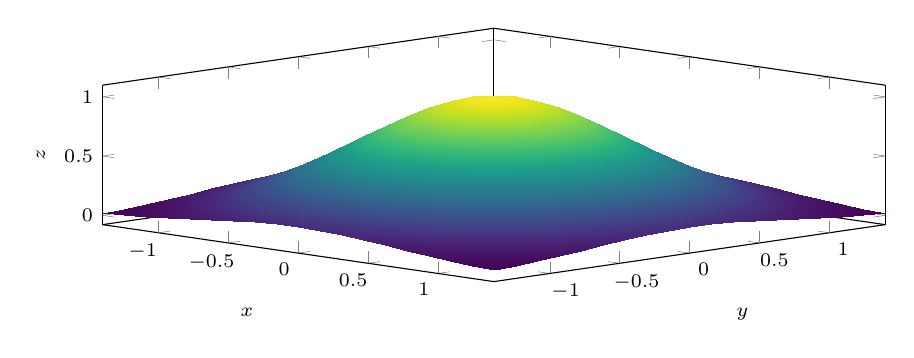
\begin{tikzpicture}
    \begin{axis}[
      width=.95\linewidth,height=48mm,
      tick label style={font=\scriptsize},label style={font=\scriptsize},
      view={45}{30},xlabel={$x$},ylabel={$y$},zlabel={$z$},
      colormap/viridis,domain=-1.4:1.4,y domain=-1.4:1.4]
      \addplot3[surf,shader=interp,samples=19,samples y=19] {exp(-x^2-y^2)};
    \end{axis}
  \end{tikzpicture}
  \caption{三维曲面}
\end{subfigure}\hfill
\begin{subfigure}[t]{0.48\textwidth}
  \centering
  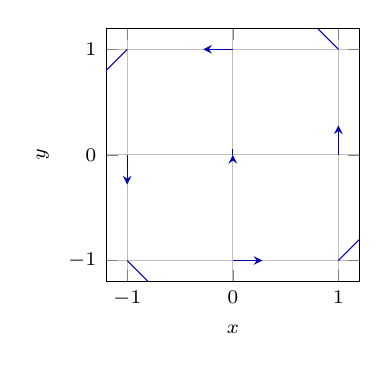
\begin{tikzpicture}
    \begin{axis}[
      width=.95\linewidth,height=48mm,
      tick label style={font=\scriptsize},label style={font=\scriptsize},
      xlabel={$x$},ylabel={$y$},xmin=-1.2,xmax=1.2,ymin=-1.2,ymax=1.2,
      axis equal image,grid=major]
      \addplot[blue!70!black,-stealth,
        quiver={u=\thisrow{u},v=\thisrow{v},scale arrows=.28}] table[row sep=crcr] {
        x y u v\\
        -1 -1 1 -1\\
         0 -1 1  0\\
         1 -1 1  1\\
        -1  0 0 -1\\
         0  0 0  0\\
         1  0 0  1\\
        -1  1 -1 -1\\
         0  1 -1  0\\
         1  1 -1  1\\
      };
    \end{axis}
  \end{tikzpicture}
  \caption{局部向量场}
\end{subfigure}

\par\medskip

\begin{subfigure}[t]{0.48\textwidth}
  \centering
  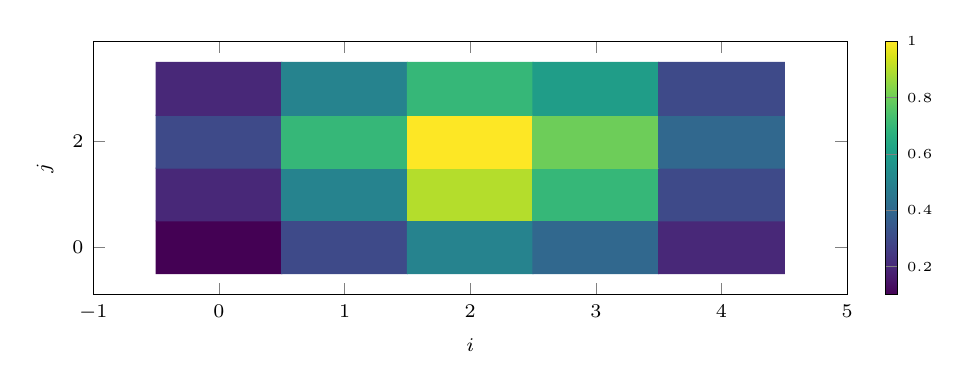
\begin{tikzpicture}
    \begin{axis}[
      tick label style={font=\scriptsize},label style={font=\scriptsize},
      width=.92\linewidth,height=48mm,
      xlabel={$i$},ylabel={$j$},view={0}{90},colorbar,colormap/viridis,
      colorbar style={width=1.5mm,tick label style={font=\tiny}}]
      \addplot[matrix plot*,mesh/cols=5,point meta=explicit] table[meta=z,row sep=crcr] {
        x y z\\
        0 0 .1\\ 1 0 .3\\ 2 0 .5\\ 3 0 .4\\ 4 0 .2\\
        0 1 .2\\ 1 1 .5\\ 2 1 .9\\ 3 1 .7\\ 4 1 .3\\
        0 2 .3\\ 1 2 .7\\ 2 2 1.0\\ 3 2 .8\\ 4 2 .4\\
        0 3 .2\\ 1 3 .5\\ 2 3 .7\\ 3 3 .6\\ 4 3 .3\\
      };
    \end{axis}
  \end{tikzpicture}
  \caption{矩阵色图}
\end{subfigure}\hfill
\begin{subfigure}[t]{0.48\textwidth}
  \centering
  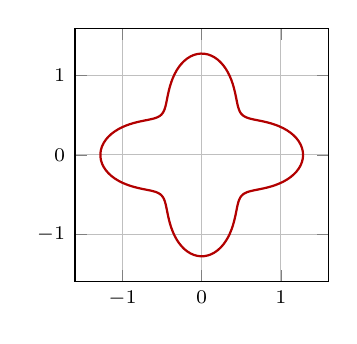
\begin{tikzpicture}
    \begin{axis}[
      width=.95\linewidth,height=48mm,
      tick label style={font=\scriptsize},label style={font=\scriptsize},
      axis equal image,grid=major,xmin=-1.6,xmax=1.6,ymin=-1.6,ymax=1.6]
      \addplot[red!70!black,thick,domain=0:360,samples=180]
        ({(1+.28*cos(4*x))*cos(x)},{(1+.28*cos(4*x))*sin(x)});
    \end{axis}
  \end{tikzpicture}
  \caption{极坐标响应}
\end{subfigure}
